\documentclass[t]{beamer}
\usepackage[english]{babel}
\usepackage[utf8]{inputenc}
\usepackage[T1]{fontenc}
\usepackage{amsmath}
\usepackage{amssymb}
\usepackage{amsfonts}
\usepackage{amsthm}
\usepackage{graphicx}
\usepackage{xcolor}
\usepackage[scaled]{helvet}
\renewcommand{\familydefault}{\sfdefault}

\usepackage{bm}
\usepackage{subcaption}
\usepackage{xcolor}
\usepackage{soul}
\usepackage{enumitem}

\usepackage[backend=biber,style=abnt,maxbibnames=3,maxcitenames=1,uniquelist=false, uniquename=full,doi,url=false]{biblatex}
\renewcommand*{\bibfont}{\scriptsizsmalle}

\AtEveryBibitem{% Clean up the bibtex rather than editing it
    \clearlist{address}
    \clearfield{date}
    \clearfield{eprint}
    \clearfield{isbn}
    \clearfield{issn}
    \clearlist{location}
    \clearfield{month}
    \clearfield{series}

    \ifentrytype{book}{}{% Remove publisher and editor except for books
	\clearlist{publisher}
	\clearname{editor}
    }
}

\usefonttheme[onlymath]{serif}
\addbibresource{../aftertext/references.bib} % Seus arquivos de referências

\newcommand{\R}{\mathbb{R}} 
\newcommand{\N}{\mathbb{N}} 

\newcommand{\highlight}[1]{%
  \colorbox{yellow!50}{$\displaystyle#1$}}

\renewcommand*\footnoterule{}

%%%
%%% Define cores
%%%
\definecolor{cinza}{HTML}{75818B}

%%%
%%% Remove a barra de navegação do Beamer
%%%
\setbeamertemplate{navigation symbols}{}

%%%
%%% Margem dos slides
%%%
\setbeamersize{text margin left=10mm,text margin right=5mm} 

%%%
%%% Redefine a fonte do título dos slides
%%%
\setbeamercolor{frametitle}{fg=cinza}
\setbeamerfont{frametitle}{series=\bfseries}
\setbeamerfont{frametitle}{size=\huge}

%%%
%%% Ajusta a posição do título dos slides e início do texto
%%%
\addtobeamertemplate{frametitle}{\vspace*{2mm}}{\vspace*{5mm}}

%%%
%%% Adiciona páginação nos slides
%%%
%%% Caso não queira, basta comentar este bloco inteiro
%%% para ocultar a paginação
%%%
\addtobeamertemplate{navigation symbols}{}{
\usebeamerfont{footline}
\usebeamercolor[fg]{footline}
}
\setbeamercolor{footline}{fg=cinza}
\setbeamerfont{footline}{series=\bfseries}
\setbeamerfont{footline}{size=\tiny}
\setbeamertemplate{footline}{
\usebeamerfont{page number in head}
\usebeamercolor[fg]{page number in head}
\hspace{5mm}
\insertframenumber/\inserttotalframenumber
\vspace{5mm}
}

%%%
%%% Redefine símbolo padrão do itemize
%%%
\setbeamertemplate{itemize items}[ball]

%%%
%%% Insere numeração nas figuras
%%%
\setbeamertemplate{caption}[numbered]

%%%
%%% Imagem de fundo a ser usada em todos os slides (exceto
%%% no primeiro e no último)
%%%
\usebackgroundtemplate
{

\includegraphics[width=\paperwidth,height=\paperheight]{fundo.png}
}

%%%
%%% Adiciona slide de "Estrutura"
%%%
\AtBeginSection[]{\frame{\frametitle{Agenda}\tableofcontents
[current]}}

%%%
%%% Define fontes e cores do slide de "Estrutura"
%%%
\setbeamerfont{section in toc}{series=\bfseries}
\setbeamercolor{section in toc}{fg=gray}
\setbeamerfont{section in toc shaded}{series=\mdseries}
\setbeamercolor{section in toc shaded}{fg=gray!01}
\setbeamercolor{subsection in toc}{fg=cinza}
\setbeamercolor{subsection in toc shaded}{fg=gray!60}
\setbeamercolor{subsubsection in toc}{fg=cinza}
\setbeamercolor{subsubsection in toc shaded}{fg=gray!60}

\mode<presentation>
%%%
%%% Início
%%%
\begin{document}

%%%
%%% Slide da capa
%%%
{
\usebackgroundtemplate{
\includegraphics[width=\paperwidth]{capa.png}}
\begin{frame}[plain]
\vspace{18mm}
%%%
%%% Título da Apresentação
%%%
\begin{flushright}
\textcolor{cinza}{\textbf{\Large{
Physics-Informed DEQs for Solving ODEs
}}}
\end{flushright}

\vspace{-6mm}
%%%
%%% Nome do autor
%%%
\begin{flushright}
\textcolor{cinza}{\textbf{\scriptsize{
Bruno M. Pacheco
}}}
\end{flushright}

\vspace{-7mm}
%%%
%%% Formação | Departamento | Centro
%%%
\begin{flushright}
\textcolor{cinza}{\scriptsize{
Defesa de Projeto de Fim de Curso | DAS
}}
\end{flushright}


\end{frame}
}

%%%
%%% Objetivo do PFC
%%%

\begin{frame}
\frametitle{Goal}
\textbf{Study}, \textbf{implement} and \textbf{validate} the use of \emph{Deep Equilibrium models} as effective and efficient solvers for IVPs, making use of \emph{physics-informed} training.

\begin{itemize}
    \item<2-> \textbf{Study} DEQs and PINNs;
    \item<3-> \textbf{Implement} a PIDEQ;
    \item<4-> \textbf{Validate} PIDEQ as an IVP solver.
\end{itemize}
\end{frame}


%%%
%%% Demais slides (exceto o slide final)
%%%
\begin{frame}
\frametitle{Agenda}
\tableofcontents
\end{frame}

\section{Background}

\subsection{Ordinary Differential Equations}

\begin{frame}
    \frametitle{Ordinary Differential Equations (ODEs)}
    ODEs describe the relationship between unknown quantities and their rates of change.
    \begin{equation}
    \frac{d \bm{y}\left( t \right) }{d t} = \mathcal{N}\left( t, \bm{y}\left( t \right)  \right) 
    \end{equation}\pause

    \emph{Initial Value Problems} (IVPs):
    \begin{align*}
	\phi :\R&\to \R^{m} \\
	\text{s.t.} \quad \frac{d \phi\left( t \right) }{d t} &= \mathcal{N}\left( t, \phi\left( t \right)  \right), t\in I \\
		    \phi(t_0) &= \bm{y}_0
    .\end{align*}
\end{frame}

\begin{frame}
    \frametitle{IVP Solvers}
    Numerical approximations $\left\{ \bm{y}_i \right\}_{i=1,\ldots}$ such that $\bm{y}_i \approx \phi(t_i)$ for $t_i \in I$. \pause

    Euler's method: \[
\bm{y}_{i+1} = \bm{y}_{i} + h\mathcal{N}\left( t_i, \bm{y}_i \right)
    \] \pause
    Runge-Kutta 4:
    \begin{align*}
	\bm{k}_1 &= \mathcal{N}\left( t_i , \bm{y}_i \right)  \\
	\bm{k}_2 &= \mathcal{N}\left( t_i+\frac{h}{2}, \bm{y}_i + \frac{h}{2}\bm{k}_1 \right)  \\
	\bm{k}_3 &= \mathcal{N}\left( t_i+\frac{h}{2}, \bm{y}_i + \frac{h}{2}\bm{k}_2 \right)  \\
	\bm{k}_4 &= \mathcal{N}\left( t_i+h, \bm{y}_i + h \bm{k}_3 \right) \\
	\bm{y}_{i+1} &= \bm{y}_i + h \frac{\bm{k}_1 + 2\bm{k}_2 + 2 \bm{k}_3 + \bm{k}_4}{6}
    \end{align*}
\end{frame}

\begin{frame}
    \begin{figure}[h]
	\vspace{.1\textheight}
	\centering
	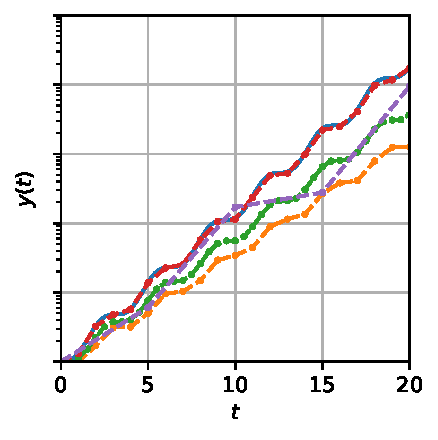
\includegraphics[width=0.45\textwidth]{../images/ode_solver_comparison_zoom.pdf}
	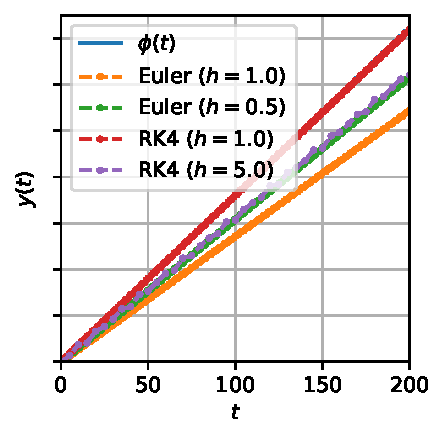
\includegraphics[width=0.45\textwidth]{../images/ode_solver_comparison.pdf}
	\caption{Comparison of Runge-Kutta 4 and Euler's method.}
	\label{fig:ode_comparison}
    \end{figure}
\end{frame}

\begin{frame}
    \frametitle{Van der Pol oscillator}
    Widely used ODE to model natural phenomena \[
    \frac{d}{dt}\begin{bmatrix} y_1\left( t \right) \\ y_2\left( t \right)  \end{bmatrix} = \begin{bmatrix} 
y_2\left( t \right) \\
\mu\left( 1-y_1\left( t \right) ^2 \right) y_2\left( t \right) - y_1(t)
\end{bmatrix} 
    ,\] where $\mu$ controls the dampening of the oscillation.

    VdP has no analytical solution \cite{panayotounakos_lack_2003}, so it is widely used as a benchmark.
    % \footnotetext{\tiny PANAYOTOUNAKOS, D.e.; PANAYOTOUNAKOU, N.d.; VAKAKIS, A.f. 2003. On the lack of analytic solutions of the Van der Pol oscillator.}
\end{frame}

\begin{frame}
    \begin{figure}[h]
	\centering
	\begin{subfigure}[b]{\textwidth}
	    \centering
	    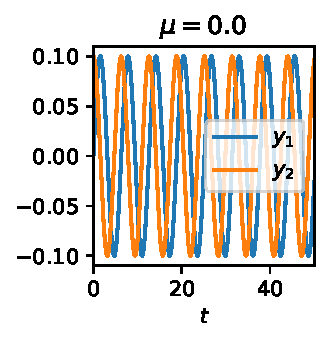
\includegraphics[width=0.3\textwidth]{../images/vdp_timeplot_mu_00.pdf}
	    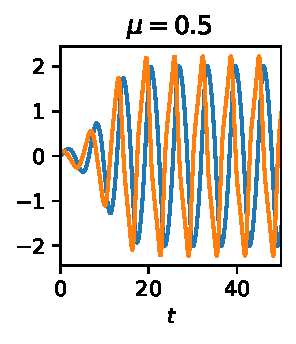
\includegraphics[width=0.27\textwidth]{../images/vdp_timeplot_mu_05.pdf}
	    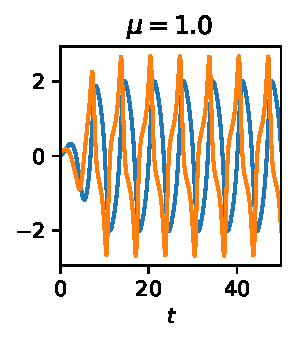
\includegraphics[width=0.27\textwidth]{../images/vdp_timeplot_mu_10.pdf}
	    %\caption{Time evolution}\label{fig:vdp_timeplots}
	\end{subfigure}
	\begin{subfigure}[b]{\textwidth}
	    \centering
	    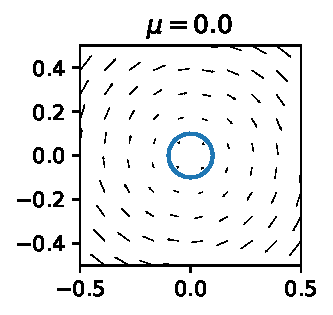
\includegraphics[width=0.3\textwidth]{../images/vdp_statespace_mu_00.pdf}
	    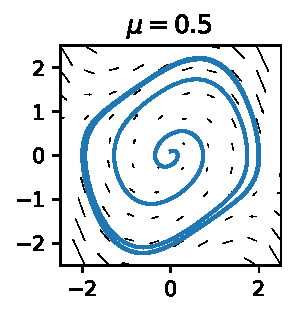
\includegraphics[width=0.27\textwidth]{../images/vdp_statespace_mu_05.pdf}
	    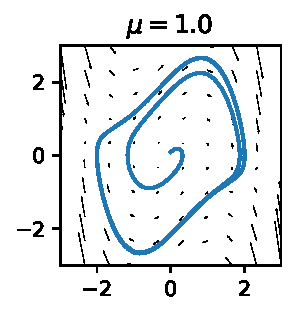
\includegraphics[width=0.27\textwidth]{../images/vdp_statespace_mu_10.pdf}
	    %\caption{State-space}\label{fig:vdp_statespace}
	\end{subfigure}
	\caption{Examples of (numerical) solutions to the Van der Pol oscillator with different dampening behavior for $\phi(0)=\bm{0}$.}\label{fig:vdp_example}
    \end{figure}
\end{frame}

\subsection{Physics-Informed Neural Networks}

\begin{frame}
    \frametitle{Physics-Informed Neural Networks}
    Let us define a neural network as a function
    \begin{align*}
	D^{FN}_{\bm{\theta}}: \R &\longrightarrow \R^{m} \\
	t &\longmapsto 	D^{FN}_{\bm{\theta}}(	t) = \bm{z}^{[L]}
    \end{align*}
    with $L$ layers such that
    \begin{align*}
	z^{[0]} &= t \\
	\bm{z}^{[i]} &= f^{[i]}_{\bm{\theta}}\left( \bm{z}^{[i-1]} \right) ,\,i=1,\ldots,L
    .\end{align*}
\end{frame}

\begin{frame}
    \frametitle{Physics-Informed Neural Networks}
    Traditionally, training such neural network on an IVP would require to optimize \[
    \min \sum_{t\in I} \|D^{FN}_{\bm{\theta}}(t) - \phi(t)\|
    ,\] 
    which would be senseless! \pause

    A PINN\cite{Raissi2019}, on the other hand, is trained on \[
    \min \sum_{t \in I} \left\|  \frac{d D^{FN}_{\bm{\theta}}(t)}{dt} - \mathcal{N}\left( t, D^{FN}_{\bm{\theta}}(t) \right) \right\| 
    ,\] 
    optimizing the \emph{dynamics} of the network.
\end{frame}

\begin{frame}
    \frametitle{Physics-Informed Neural Networks}
    More precisely, the training is on \[
	\min_{\bm{\theta}} J_b\left( \bm{\theta} \right) + \lambda J_{\mathcal{N}}\left( \bm{\theta} \right)
    ,\] with
    \begin{align*}
	J_b\left( \bm{\theta} \right) &= \|D^{FN}_{\bm{\theta}}\left( t_0 \right) -\bm{y}_0\| \\
	J_{\mathcal{N}}\left( \bm{\theta} \right) &= \sum_{t \in X_{\mathcal{N}}} \left\| \frac{d D^{FN}_{\bm{\theta}}\left( t \right) }{dt} - \mathcal{N}\left( t,D^{FN}_{\bm{\theta}}\left( t \right)  \right)  \right\|
    ,\end{align*}
    in which $X_{\mathcal{N}}\subset I$ is a set of random points from the domain.
\end{frame}

\begin{frame}
    \begin{figure}[h]
        \centering
        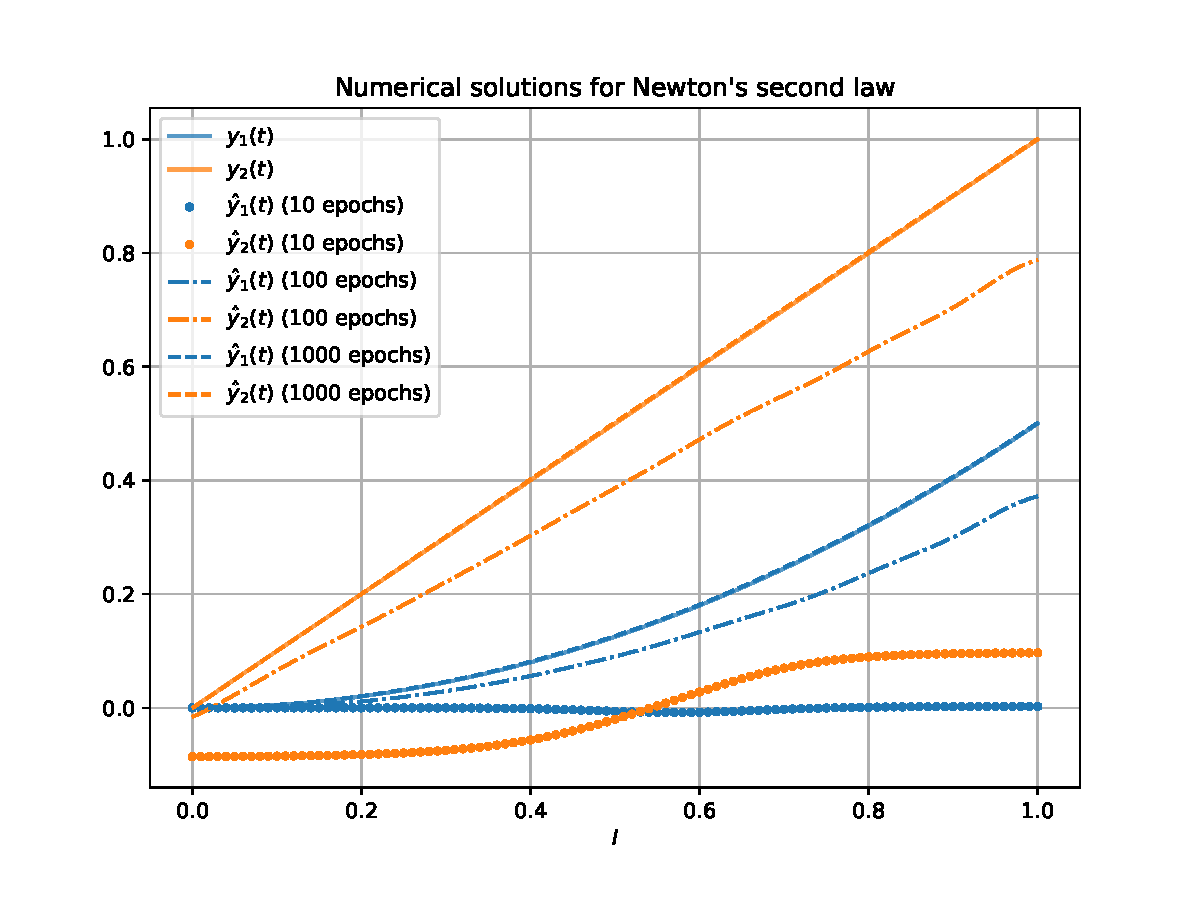
\includegraphics[width=0.8\textwidth]{../images/pinn_newton.pdf}
        \caption{Example of PINN trained to solve IVP of Newton's second law with $y(0)=0$ and constant force. $y_1$ is the velocity and $y_2$ is the acceleration.}
        \label{fig:-images-pinn_newton-pdf}
    \end{figure}
\end{frame}

\subsection{Deep Equilibrium Models}

\begin{frame}
    \frametitle{Deep Equilibrium Models}
    \begin{columns}
	\column{0.5\textwidth}
	Deep Feedforward Network:
	\begin{align*}
	    D^{FN}_{\bm{\theta}}: \R &\longrightarrow \R^{m} \\
	    t &\longmapsto 	D^{FN}_{\bm{\theta}}(	t) = \bm{z}^{[L]} \\
	    z^{[0]} &= t \\
	    \bm{z}^{[i]} &= f^{\highlight{[i]}}_{\bm{\theta}}\left( \bm{z}^{[i-1]} \right) , i\highlight{=1,\ldots,L}
	\end{align*} \pause
	\column{0.5\textwidth}
	Deep Equilibrium \hl{Model}:
	\begin{align*}
	    D^{EQ}_{\bm{\theta}}: \R &\longrightarrow \R^{m} \\
	    t &\longmapsto 	D^{EQ}_{\bm{\theta}}(	t) = \bm{z}^{[\infty]} \\
	    z^{[0]} &= t \\
	    \bm{z}^{[i]} &= f_{\bm{\theta}}\left( \bm{z}^{[i-1]} \right) , i\highlight{\to \infty}
	\end{align*}
    \end{columns}
\end{frame}

\begin{frame}
    \frametitle{Deep Equilibrium Models}
    $\bm{z}^{[\infty]}$ exists (and is well-defined) iff $\bm{z}^{[i]}$ converges.
    \linebreak \pause

    Then, $\exists N\in \N$ such that $\forall i\ge N,\,z^{[i]}\approx z^{[i+1]}$.
    \linebreak \pause

    Therefore, $\bm{z}^{\star}=\bm{z}^{[N]}\approx \bm{z}^{[\infty]}$,
    \linebreak \pause

    and $\bm{z}^{\star}$ is an \emph{equilibrium point} of $f_{\bm{\theta}}$ \[
	    \bm{z}^{\star} = f_{\bm{\theta}}\left( \bm{z}^{\star} \right)
    .\] 
\end{frame}

\begin{frame}
    \frametitle{Deep Equilibrium Models}
    Definition \cite{Bai2019}:
    \begin{align*}
	D^{EQ}_{\bm{\theta}}: \R &\longrightarrow \R^{m} \\
	t &\longmapsto 	D^{EQ}_{\bm{\theta}}(	t) = \bm{z}^{\star} \\
	\bm{z}^{\star} &= f_{\bm{\theta}}\left( t, \bm{z}^{\star} \right)
    .\end{align*}
\end{frame}

\begin{frame}
    \frametitle{Forward Pass}
    $\bm{z}^{\star}$ is an equilibrium of $f_{\bm{\theta}}$ iff $\bm{z}^{\star}$ is a root of $g_t(\bm{z}) = f_{\bm{\theta}}(t,\bm{z}) - \bm{z}$.
    \linebreak \pause

    Therefore, \[
    D^{EQ}_{\bm{\theta}}(t) = \bm{z}^{\star} = RootFind(g)
    ,\] in which $RootFind$ is any root-finding algorithm (e.g., simple iteration, Newton's method, quasi-Newton methods).
\end{frame}

\begin{frame}
    \frametitle{Backward Pass}
    By the definition of the model's output, \[
	f_{\bm{\theta}}(t,D^{EQ}_{\bm{\theta}}(t)) = 0
    ,\] i.e., $D^{EQ}_{\bm{\theta}}$ is a \emph{parametrization} of $z$ with respect to $t$.
    \linebreak \pause

    By the implicit function theorem \cite{Bai2019}, \[
	\frac{d D^{EQ}_{\bm{\theta}}(t)}{d \bm{\theta}} = - \left[ \frac{d f_{\bm{\theta}}(t,D^{EQ}_{\bm{\theta}}(t))}{d \bm{z}} - I \right]^{-1} \frac{d f_{\bm{\theta}}(t,D^{EQ}_{\bm{\theta}}(t))}{d \bm{\theta}}
    .\] 
\end{frame}

\begin{frame}
    \frametitle{Backward Pass}
    We avoid the matrix inversion, however, by computing the solution to the vector-Jacobian product \[
    \bm{v}^T = \bm{u}^T\left[ \frac{d \bm{f}_{\bm{\theta}}}{d \bm{z}} - I \right]^{-1}
    \] by finding the equilibrium point of \[
    \bm{v}^T = \bm{v}^T \frac{d \bm{f}_{\bm{\theta}}}{d \bm{z}} - \bm{u}^T
    ,\] using once again a root-finding algorithm.
    
\end{frame}

\section{Experiments and Results}

\subsection{PIDEQ}

\begin{frame}
    \frametitle{PIDEQ}
    We propose a model 
    \begin{align*}
	D^{EQ}_{\bm{\theta}}: \R &\longrightarrow \R^{m} \\
	t &\longmapsto 	D^{EQ}_{\bm{\theta}}(	t) = \highlight{C} \bm{z}^{\star} \\
	\bm{z}^{\star} &= f_{\bm{\theta}}\left( t, \bm{z}^{\star} \right)= \highlight{\tanh \left( A\bm{z} + t\bm{a} + \bm{b} \right)}
    \end{align*}
    trained to \[
     \min_{\bm{\theta}} J_b\left( \bm{\theta} \right) + \lambda J_{\mathcal{N}}\left( \bm{\theta} \right) + \kappa \highlight{\left\lVert \frac{d f_{\bm{\theta}}}{d \bm{z}}\right\rVert_F}
    .\] \pause
    
    \textcolor{red}{In a DEQ, optimizing $J_{\mathcal{N}}$ requires the backward pass' root-finding algorithm to be differentiable.}
\end{frame}

\subsection{Experiments}

\begin{frame}
    \frametitle{Baseline Results}
    PINN based on \textcite{Antonelo2021} (4 layers of 20 nodes) and PIDEQ from the theoretical results of \textcite{Ghaoui2019} (80 states).

    \begin{figure}[h]
	\centering
	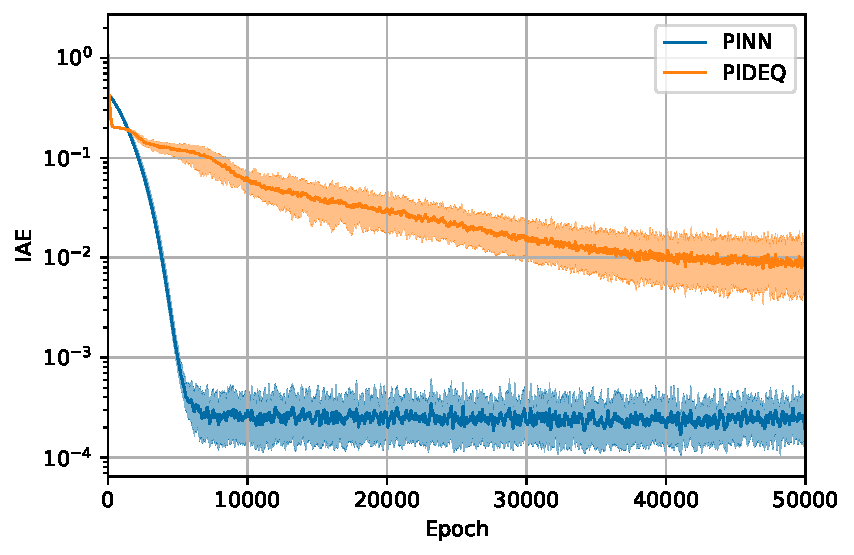
\includegraphics[width=0.6\textwidth]{../images/exp_1_iae.pdf}
	\caption{Learning curves of the baseline models.}
	\label{fig:baseline-iae}
    \end{figure}
\end{frame}

\begin{frame}
    \frametitle{PIDEQ Size}
    The resulting PIDEQ seems unnecessarily big, with too many states.
    \begin{figure}[h]
	% \centering
	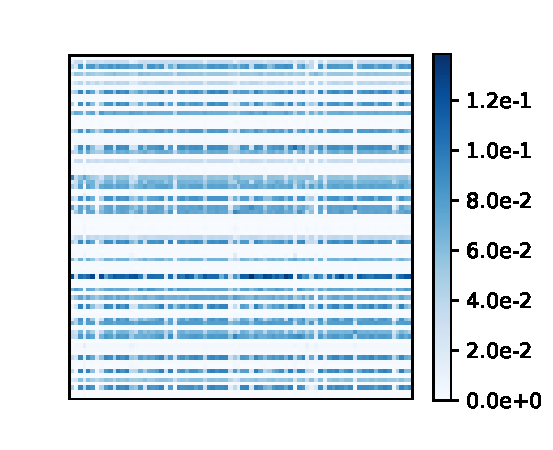
\includegraphics[width=.4\textwidth]{../images/exp_1_matplot.pdf}
	\caption{$A$ matrix of the baseline PIDEQ (80 states) after training.}
	\label{fig:baseline-pideq-A}
    \end{figure}
\end{frame}

\begin{frame}
    \frametitle{PIDEQ Size}
    \begin{columns}[c]
    \begin{column}{.4\textwidth}
	This motivated the training of smaller PIDEQs, iterating over the analysis on the $A$ matrix.
    \end{column}
    \begin{column}{.6\textwidth}
	\begin{figure}[h]
	    \centering
	    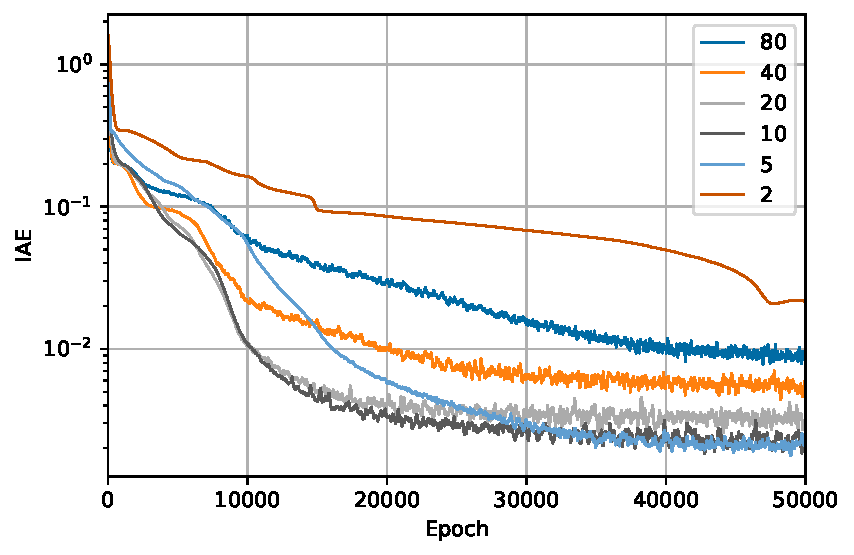
\includegraphics[width=\textwidth]{../images/exp_2_iae.pdf}
	    \caption{Learning curves of the models trained with fewer states.}
	    \label{fig:states-iae}
	\end{figure}
    \end{column}
    \end{columns}
\end{frame}

\begin{frame}
    \frametitle{Hyperparameter Tuning}

    \begin{columns}[c]
    \begin{column}{.4\textwidth}
	Besides the number of states, we also tuned:
	\begin{itemize}[label={\textbullet}]
	    \item<1-> Weight of the Jacobian regularization term ($\kappa$);
	    \item<2-> Root-finding algorithm used in the forward pass;
	    \item<3-> Tolerance of the root-finding algorithms ($\varepsilon$).
	\end{itemize}
    \end{column}
    \begin{column}{.6\textwidth}
	\only<1>{\begin{figure}[h]
            \centering
            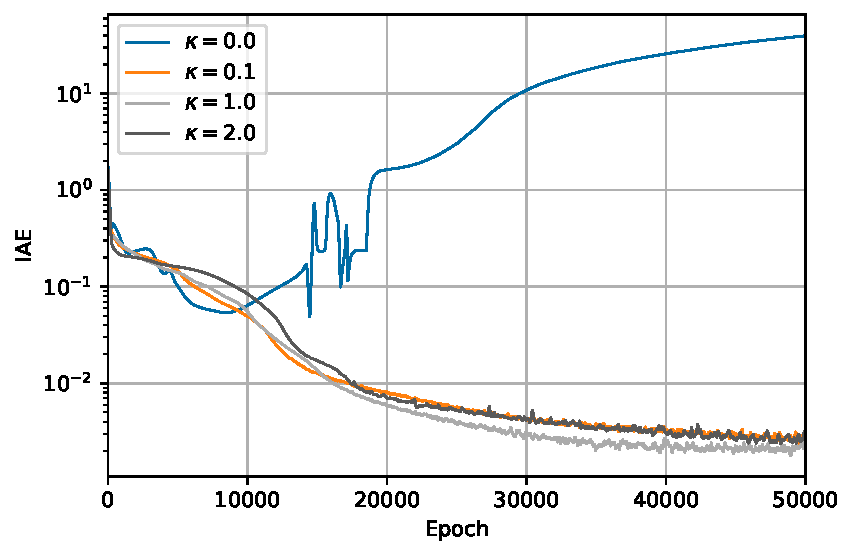
\includegraphics[width=1.\textwidth]{../images/exp_4_iae.pdf}
            \caption{Learning curves of the models trained with different $\kappa$.}
            \label{fig:kappa-iae}
	\end{figure}}
        \only<2>{\begin{figure}[h]
            \centering
            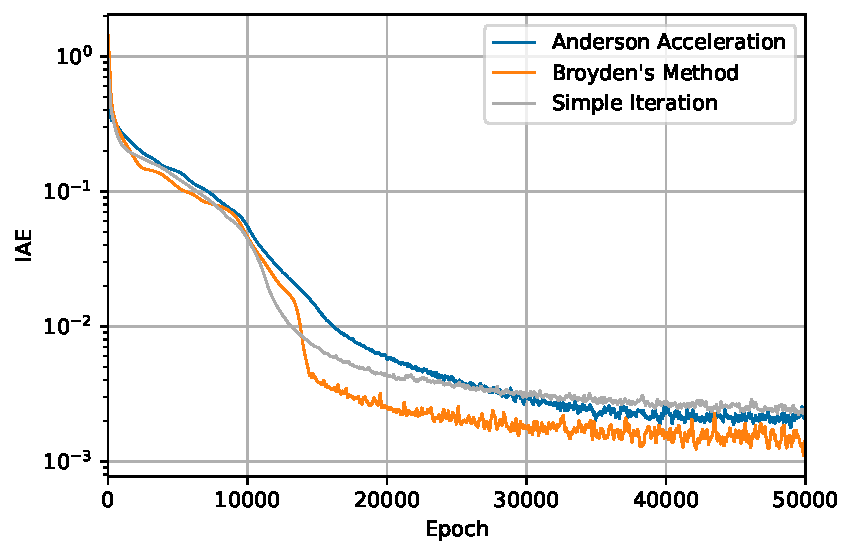
\includegraphics[width=\textwidth]{../images/exp_5_iae.pdf}
            \caption{Learning curves of the models trained with different root-finding algorithms.}
            \label{fig:solver-iae}
	\end{figure}}
        \only<3>{\begin{figure}[h]
            \centering
            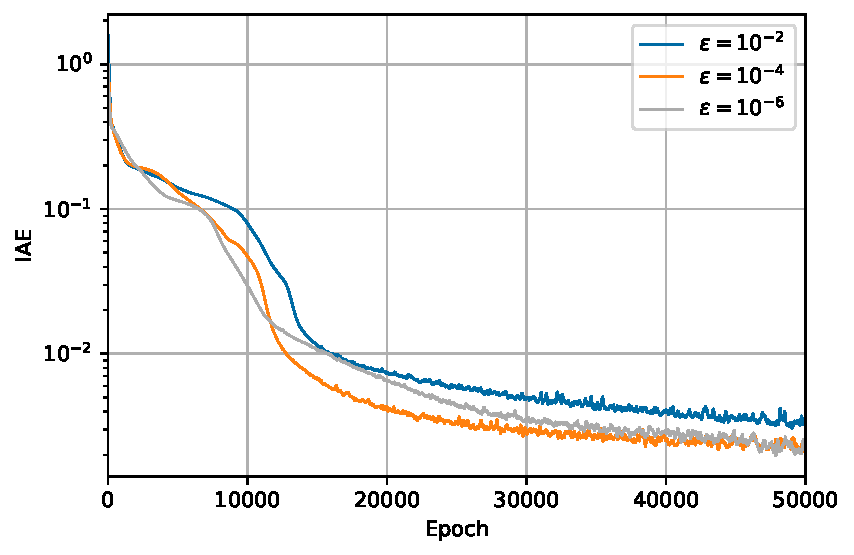
\includegraphics[width=\textwidth]{../images/exp_6_iae.pdf}
            \caption{Learning curves of the models trained with different $\varepsilon$.}
            \label{fig:solver-iae}
	\end{figure}}
    \end{column}
    \end{columns}
\end{frame}

\begin{frame}
    \frametitle{Final Model}
    Besides the tuned PIDEQ, a PINN with the same number of parameters was trained for a fair comparison.
    \begin{figure}[h]
	\centering
	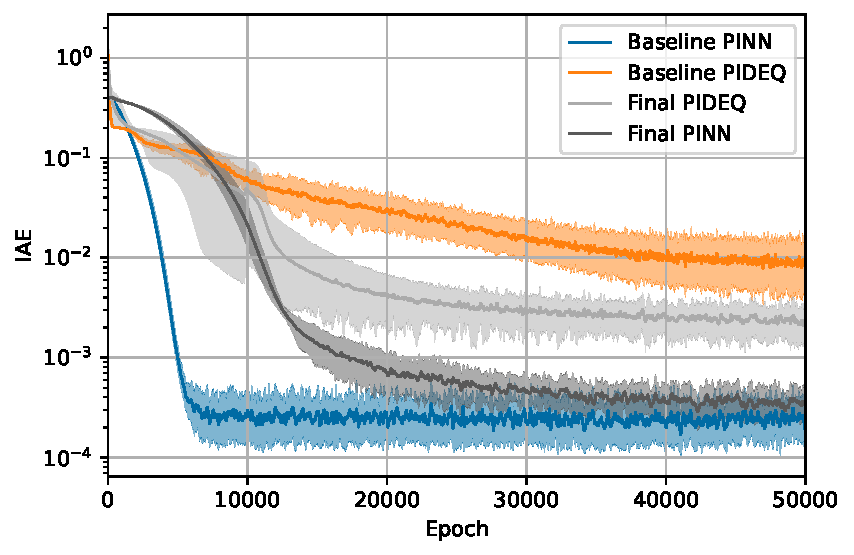
\includegraphics[width=.6\textwidth]{../images/final_iae.pdf}
	\caption{Learning curve of the final models and the baselines. ``Final PINN'', ``Final PIDEQ'' have 52 parameters.}
	\label{fig:final-iae}
    \end{figure}
\end{frame}

\begin{frame}
    % \frametitle{Final Model}
    \begin{figure}[h]
	\vspace{.1\textheight}
	\centering
	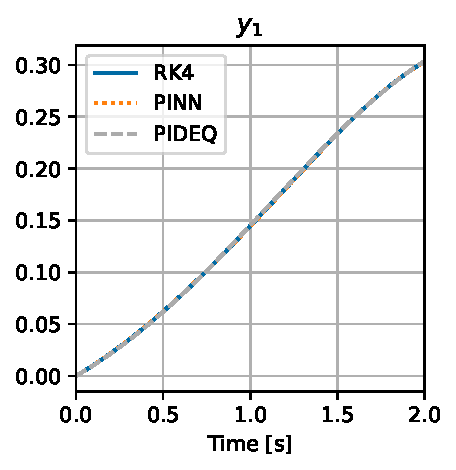
\includegraphics[width=.45\textwidth]{../images/final_vdp_y1.pdf}
	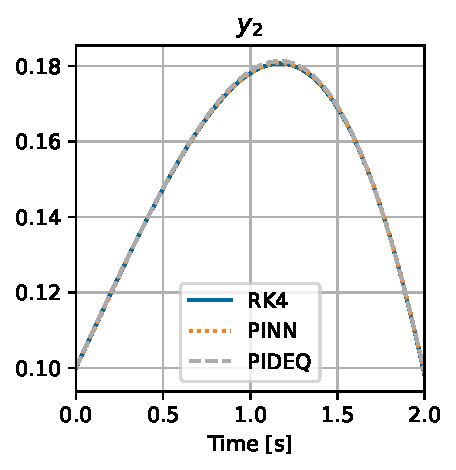
\includegraphics[width=.45\textwidth]{../images/final_vdp_y2.pdf}
	\caption{Prediction of PINN and PIDEQ in comparison to the reference approximation resulting from RK4.}
	\label{fig:final-vdp}
    \end{figure}
\end{frame}

\begin{frame}
    \frametitle{Final Model}
    \begin{columns}[T] 
	\begin{column}{.6\textwidth}
	    \vspace{-10pt}
	    \begin{figure}[h]
	        \centering
		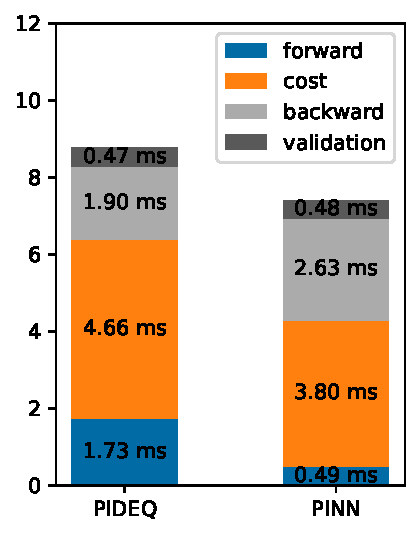
\includegraphics[width=.6\textwidth]{../images/final_times.pdf}
		\caption{Breakdown of median time per epoch for the final PIDEQ and PINN.}
		\label{fig:final-times}
	    \end{figure}
        \end{column}
	\begin{column}{.4\textwidth} 
	    \begin{description}
	        \item[forward] computing the output given the input during training;
		\item[cost] computing the cost function;
		\item[backwards] back-propagating the cost to the parameters;
		\item[validation] computing the output during validation (inference).
	    \end{description}
	\end{column}
    \end{columns}
    
\end{frame}

\section{Discussion}

\subsection{Conclusions}

\begin{frame}
    \frametitle{Conclusions}
    \begin{itemize}[label={\textbullet}]
        \item<1-> It is possible to train DEQs in a physics-informed manner, effectively solving IVPs of ODEs;
	\item<2-> However, PIDEQs are slower to train and presented higher errors than PINNs in comparison to RK4;
	\item<3-> We believe that this might be because IVPs of small ODEs do not benefit from deeper networks;
    \end{itemize}
\end{frame}

\subsection{Outlook}

\begin{frame}
    \frametitle{Outlook}
    \begin{itemize}[label={\textbullet}]
	\item<1-> More complex problems, that benefit from deeper networks, might be a better use case for PIDEQs (e.g., IVP of the 4 Tank system \cite{johansson_quadruple-tank_2000-1}, IVPs of PDEs \cite{Raissi2019}, state-informed/controllable PINNs \cite{Antonelo2021,Arnold2021});
	\item<2-> In theory, the implicit function theorem can be further exploited to find higher-order derivatives of DEQs, eliminating the requirement for differentiable root-finding algorithms.
    \end{itemize}
\end{frame}

%%%
%%% Slide final
%%%
{
\usebackgroundtemplate{
\includegraphics[width=\paperwidth]{capa.png}}
\begin{frame}[plain]
\vspace{15mm}
\begin{center}
\textcolor{cinza}{
\textbf{Obrigado pela Atenção}
}
\end{center}
\vspace{-6mm}
\begin{center}
\textcolor{cinza}{\scriptsize{
	Bruno M. Pacheco
}}
\end{center}
\vspace{-6mm}
\begin{center}
\textcolor{cinza}{\scriptsize{
mpacheco.bruno@gmail.com
}}
\end{center}
\vspace{-6mm}
\begin{center}
\textcolor{cinza}{\scriptsize{
\href{https://github.com/brunompacheco/pideq}{github.com/brunompacheco/pideq}
}}
\end{center}
\end{frame}
}

\begin{frame}[allowframebreaks]
    \frametitle{References}
    \printbibliography
\end{frame}

\end{document}

